Moving forward, there are several improvements that can be made to the 2D/1D scheme with regard to the cusping problem.  Four of these improvements will be discussed in this section.  The first two are modifications to methods already in MPACT, while the second two would involve implementation of new solvers.

\section{Improvements to Sub-Plane--Based Decusping techniques}

The sub-plane--based decusping solvers presented in chapters \ref{chap:cusping}-\ref{chap:results} are capable of reducing the cusping errors significantly over having no treatment.  They also provide a more general solution to the problem than the polynomial corrections that existed in MPACT previously.  However, there are at least two improvements that can be made going forward.  The first deals with approximations made in the calculation of the radial currents, and the second deals with the auxiliary solver used to generate the radial flux profiles.

\subsection{Radial Transverse Leakage Source}

The current implementation of the sub-plane scheme assumes the same $\hat{D}$ current correction term for all sub-plane surfaces between two pin cells.  This assumption is made to improve the stability of the sub-plane scheme, but certainly introduces some error in the CMFD and SP$_3$ calculations.  In most cases, this error is likely quite small, since the axial shape of the solution usually changes gradually.  However, when a control rod is partially inserted into an MOC plane, the currents in the rodded sub-planes are much different from those in the unrodded sub-plane.  The CMFD calculations predict that this is the case, but using the same $\hat{D}$ for both of these regions likely introduces a more significant error than for other regions of the problem.  Moving forward, work will be done to develop sub-plane--dependent $\hat{D}$ terms to improve the accuracy of the radial TL source for the SP$_3$ solver.

\subsection{Auxiliary Solver}

Another potential source of error for the decusping treatments discussed here is in the choice of auxiliary solver.  The 1D CP kernel was useful for capturing some of the radial cusping effects, but it does have some deficiencies.  First, because it is 1D, it ignores the corner effects of the pin cell by treating the moderator as a ring.  This minimizes the directional dependence of the neutrons, changing the radial flux profile generated by the solver.  Second, the 1D CP solver relies on a buffer region obtained by homogenizing the surrounding pin cells.  As with the moderator region, this buffer region is assumed to be annular and homogeneous.  This affects the source term which drives the problem and the behavior of the neutrons which escape the pin cell of interest.  To eliminate these problems, a different method could be used in place of the 1D CP solver.  

One alternative method that would resolve both of the deficiencies mentioned here would be a highly optimized 2D MOC solver.  Using 2D MOC, an octant-symmetric pin cell could be simulated quickly, capturing the effects of the corner on the flux in the pin cell.  Furthermore, the boundary conditions could be handled several different ways.  The first would be to simply have an isotropic incoming angular flux calculated from the radial currents generated by the planar MOC calculations.  Another option would be to explicitly store the incoming angular fluxes along the surfaces of the partially rodded pin cell during the planar MOC calculation.  A third way of dealing with the boundary conditions would be simulate the neighboring cells as well.  Doing this would allow use of isotropic angular flux boundary conditions on the neighbor's boundary while still having an angular shape upon reaching the partially rodded cell.  This third option would allow the 2D MOC solver to improve on the 1D CP solver without any modifications to the 2D planar MOC calculations.

\section{Sub-Ray Method of Characteristics}

While the current methods can be improved in the near term, they still are not able to fully resolving the rod cusping issue in the long run.  This section will describe some of the circumstances in which the decusping techniques described in this work will either provide inaccurate results or fail altogether.  After this, some results will be presented from a 1D MOC code to show the effects of cross-section homogenization on the angular flux.  Finally, a new way of performing MOC calculations will be presented.  This method will provide a fully general way of dealing with axial material heterogeneities in 2D/1D by directly addressing the angular flux, which is a more fundamental quantity than the scalar flux.  Additionally, a timeline for the development, implementation and testing of this method will be included.

\subsection{Motivation}

\begin{enumerate}[leftmargin=*]
  \item CE Rods
  \item BWR Control Blades
  \item Fundamentally just correcting things after the fact
\end{enumerate}

\subsection{1D MOC Results}

To analyze the behavior of the angular flux in relationship to homogenized cross-sections, a 1D MOC code was written that could solve eigenvalue and fixed source problems.  This code was used to solve a 1D variation of VERA Problem 4.  The center row of pins across all three problems were modeled in the 1D code.  The pin pitch of 1.26 cm was maintained and the volume fractions of each material in the actual Problem 4 were used to calculate the thicknesses of each region.  The 1D model of the center assembly had 4 guide tubes and one instrument tube, while the other two assemblies had only empty guide tubes.

The four guide tubes in the center assembly could be modified to be a mixture of moderator and control rod material.  Changing this mixture and running different calculations provides some insight into the effects of the cross-section homogenization on the angular flux.  Each of these calculations used cross-sections from the C5G7 benchmark \todo{cite}.

\subsubsection{Specified Source}

The first calculations that were performed used a mixture that was 50\% control rod and 50\% moderator by volume.  First, a full eigenvalue calculation was performed to obtain a fission and scattering source distribution for the whole model.  Once this was completed, a single MOC sweep was performed using the 50-50 cross-section mixture, 100\% rodded cross-section, and 100\% moderator cross-section.  Figure \ref{f:1dmoc-fixed-50-scalflux7} shows the group 7 scalar flux for this calculation, and Figure \ref{f:1dmoc-fixed-50-angflux}

\begin{figure}[h]
    \centering
    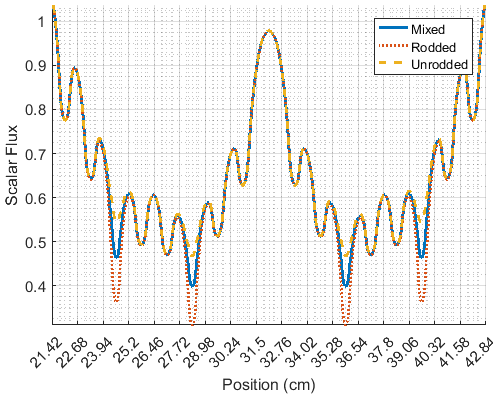
\includegraphics[width=0.8\textwidth]{../figs/1dmoc-50mix-fixedscat-scalflux7.png}
    \caption{Group 7 scalar flux comparisons for a fixed fission and scattering source calculation}\label{f:1dmoc-fixed-50-scalflux7}
\end{figure}

\begin{figure}[h]
    \centering
    \subfigure[Group 1]{
        \centering
        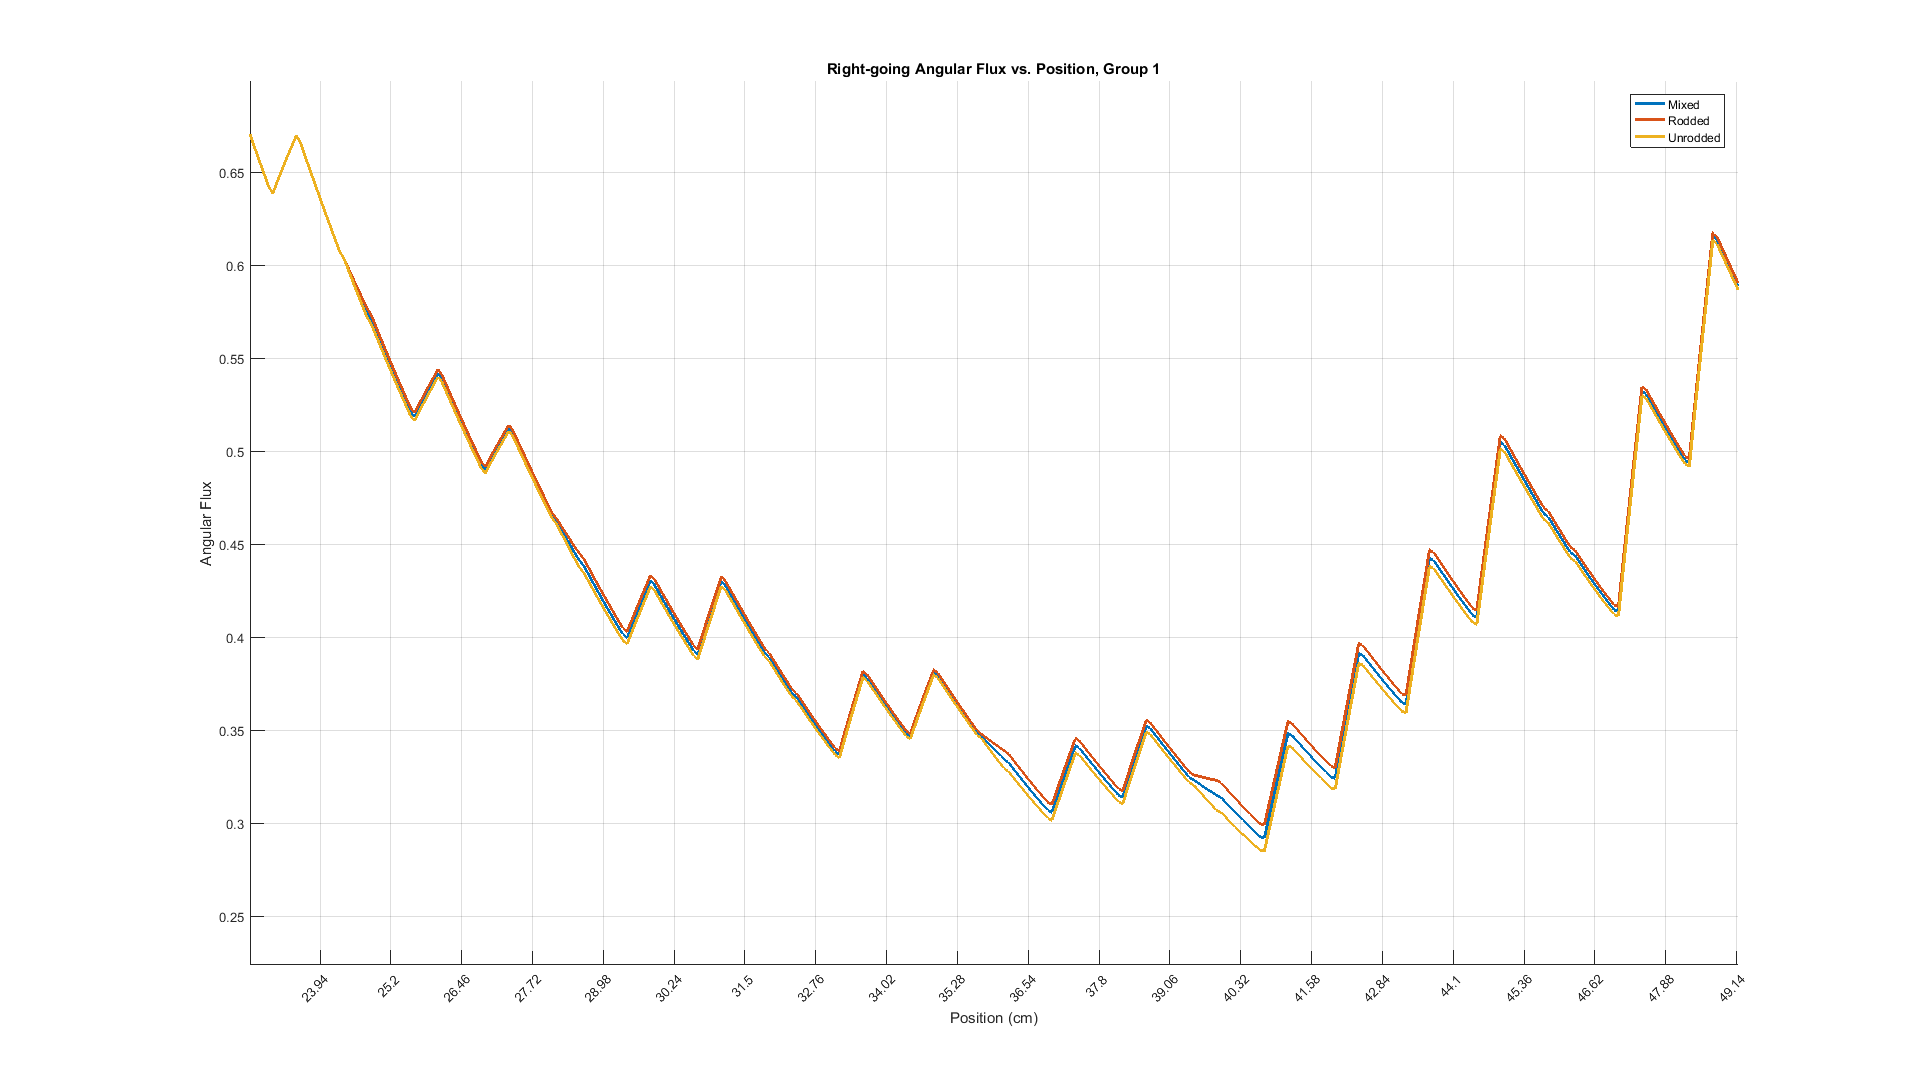
\includegraphics[width=0.45\textwidth]{../figs/1dmoc-50mix-fixedscat-angflux1.png}
        \label{f:1dmoc-fixed-50-angflux1}
    }
    ~
    \subfigure[Group 7]{
        \centering
        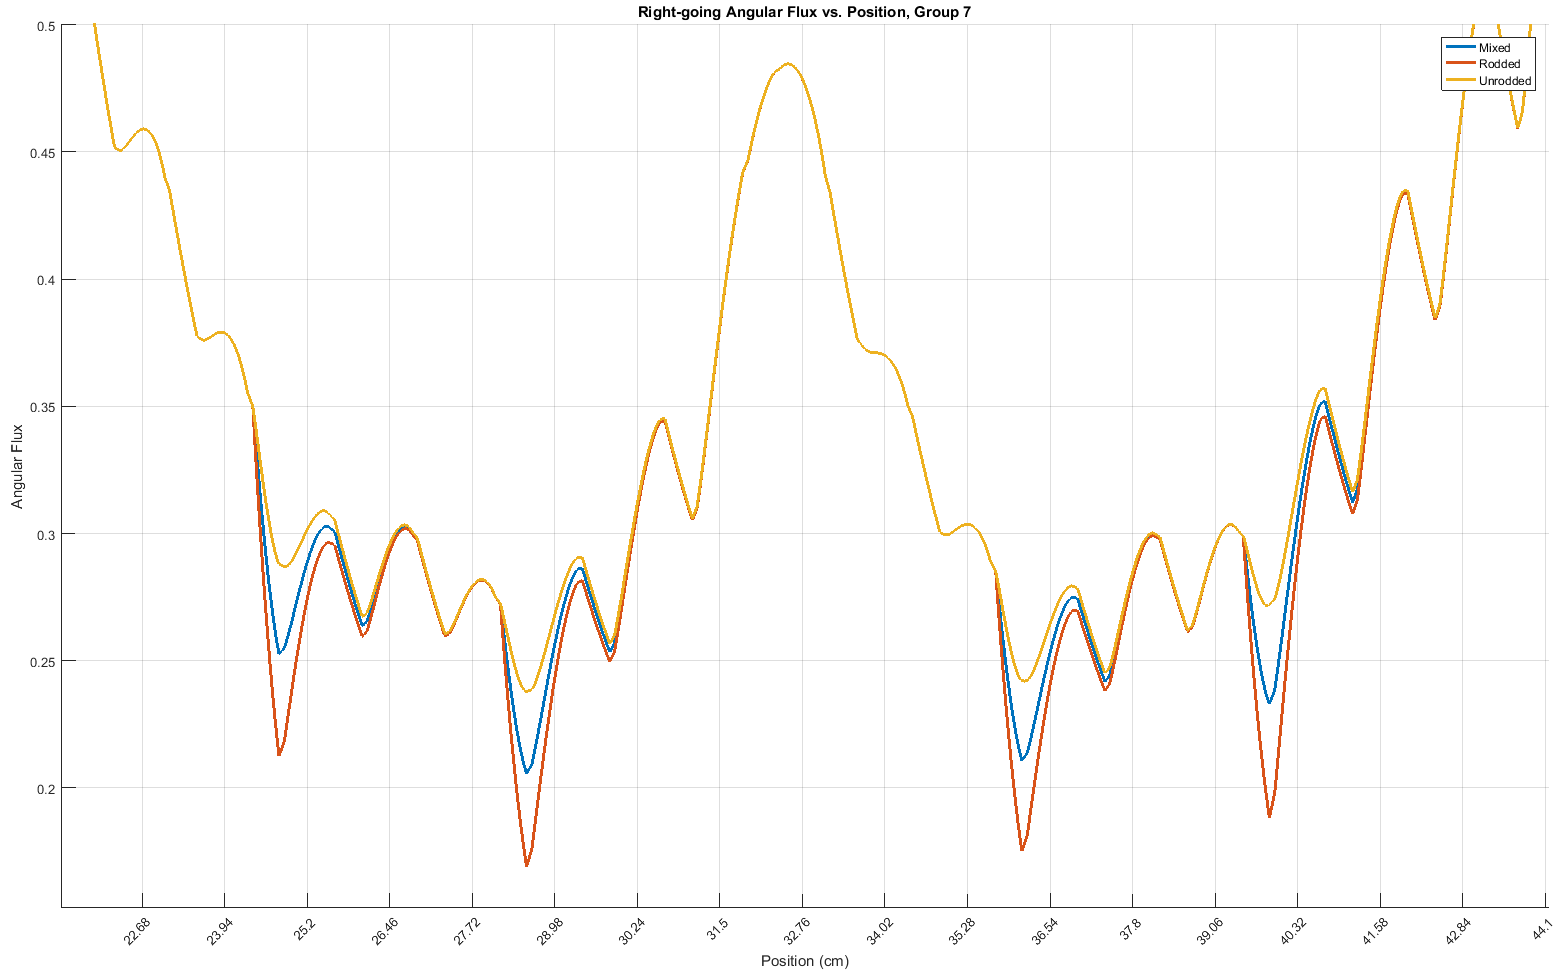
\includegraphics[width=0.45\textwidth]{../figs/1dmoc-50mix-fixedscat-angflux7.png}
        \label{f:1dmoc-fixed-50-angflux7}
    }
    \caption{Angular flux comparisons for a fixed fission and scattering source calculation}\label{f:1dmoc-fixed-50-angflux}
\end{figure}

\subsubsection{Fixed Fission Source}

\begin{figure}[h]
    \centering
    \subfigure[25\% Mixture]{
        \centering
        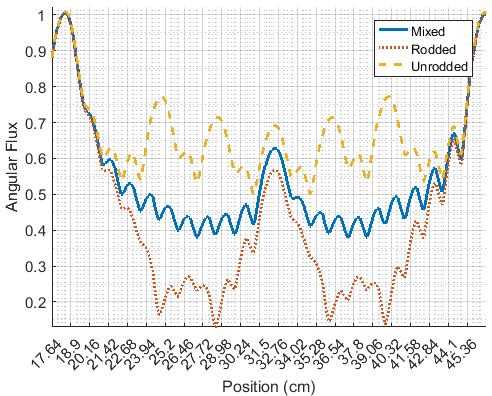
\includegraphics[width=0.45\textwidth]{../figs/1dmoc-25mix-angflux7.png}
        \label{f:1dmoc-25-angflux7}
    }
    ~
    \subfigure[50\% Mixture]{
        \centering
        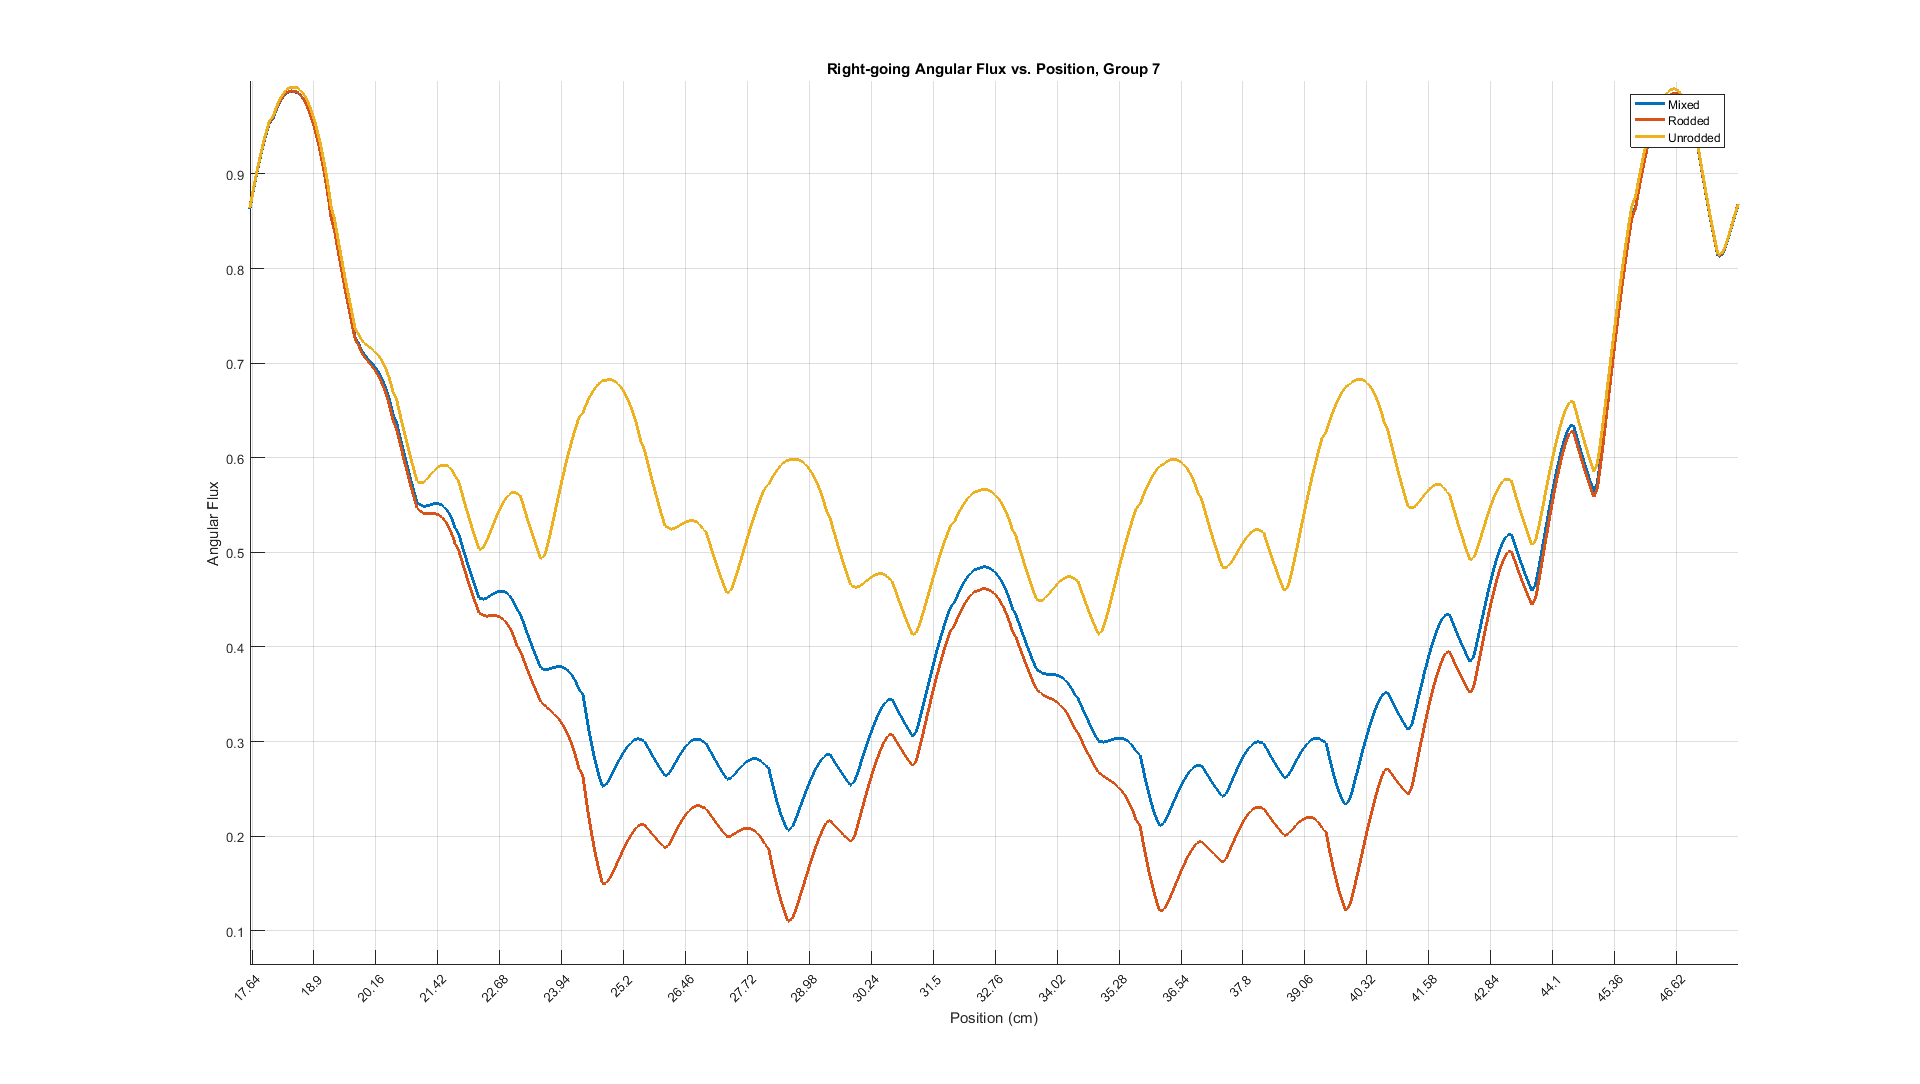
\includegraphics[width=0.45\textwidth]{../figs/1dmoc-50mix-angflux7.png}
        \label{f:1dmoc-50-angflux7}
    }
    ~
    \subfigure[75\% Mixture]{
        \centering
        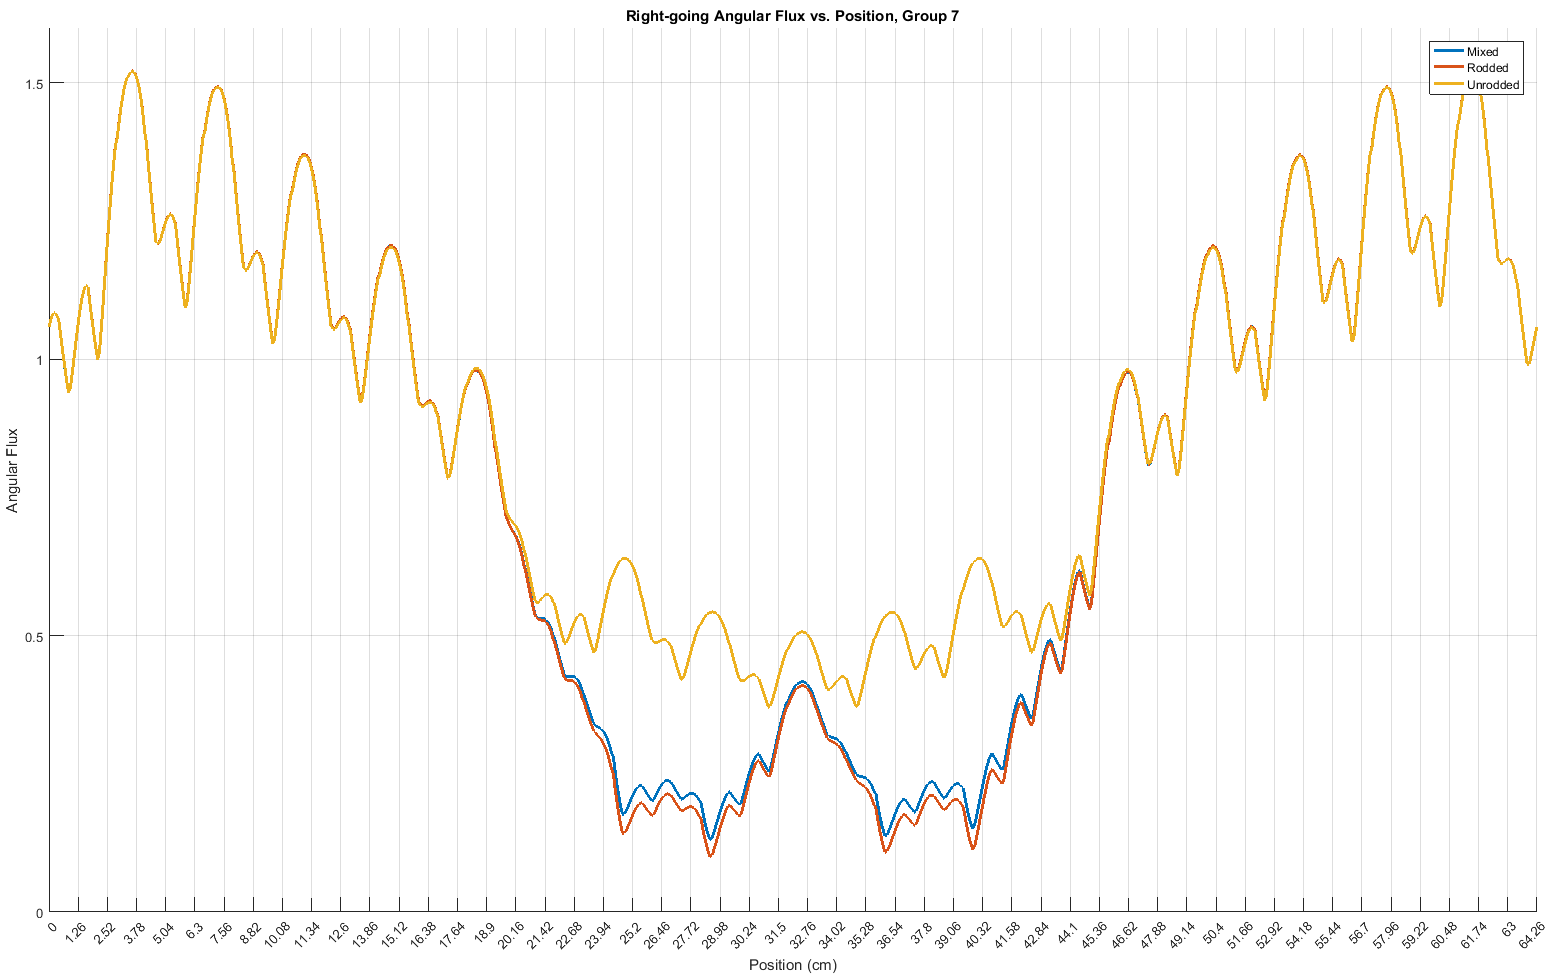
\includegraphics[width=0.45\textwidth]{../figs/1dmoc-75mix-angflux7.png}
        \label{f:1dmoc-75-angflux7}
    }
    \caption{Group 7 angular flux comparisons for 25\% and 75\% mixtures}\label{f:1dmoc-angflux7}
\end{figure}

\begin{enumerate}[leftmargin=*]
  \item Done - Describe problem 4 model
  \item Done - Describe procedure for 1-inner calculations
  \item Done - Present results
  \item Discuss range of effects on angular flux
  \item Describe procedure for full FSP
  \item Present Results - Mostly done.  Show one fast flux plot to show it's mainly just the thermal groups we care about.
  \item Discuss the difference between the sources exposed by the different flux shapes
\end{enumerate} 

\subsection{Sub-Ray MOC Method Description}

\begin{enumerate}[leftmargin=*]
  \item Explain method concept -- Maybe a diagram of fuel, partial CR, fuel to show how the ray splitting/combining looks
  \item Need different XS and sources - use subplane
  \item Has to work well with axial solver - RTL improvements
  \item Timeline
\end{enumerate}